\chapter{ Chapitre 8 : Sprint 5 "Recherche des données sur un Map, \centering Gestion des tableaux de bord et des Messageries"}
\begin{spacing}{1.2}
\minitoc
\thispagestyle{MyStyle}
\end{spacing}
\newpage
\begin{sloppypar} 

\section{Introduction}
\vspace{-4mm}
Dans ce sprint, nous améliorons la communication entre l'administration et les étudiants via un chat dashboard dans la partie web admin. De plus, nous ajoutons une carte interactive pour guider les étudiants. Ces améliorations visent à faciliter la communication et à offrir une expérience utilisateur plus intuitive. 
\vspace{-8mm}

\section{Backlog du sprint}
\vspace{-4mm}
Le backlog pour le chat, le tableau de bord et la carte inclut des fonctionnalités telles que la mise en place d'un système de messagerie instantanée entre l'administrateur et les utilisateurs, le développement d'un tableau de bord pour afficher des données clés et la création d'une carte interactive pour aider les utilisateurs à naviguer et à trouver des informations pertinentes. Ces fonctionnalités visent à améliorer l'expérience utilisateur et à fournir des outils efficaces pour la gestion et la visualisation des données.

\begin{table}[h]
\centering
\begin{tabular}{|p{9cm}|p{3cm}|p{3cm}|}
\hline
\textbf{ Tâches } & \textbf{ Priorité }& \textbf{Période/jour}  \\
\hline
En tant qu’un étudiant ,je peux contacter l’administrateur.& Élevée  & 5 jours \\
\hline
En tant qu'un étudiant , je peux contacter l’administrateur sur l'application mobile.  & Élevée  & 4 jours  \\
\hline
En tant qu’un administrateur, je peux consulter le tableau de bord dans l’application web & Élevée  & 7 jours  \\
\hline
En tant qu’un utilisateur ,je peux consulter la carte map sur l'application mobile  & Élevée  & 7 jours  \\
\hline

\end{tabular}
\caption{Tableau de Backlog de produit Sprint 5}
\end{table}
\vspace{-1cm}
\section {Analyse et spécification des besoins}
\vspace{-4mm}
Afin de mieux comprendre la structure de notre système, nous avons utilisé un diagramme de cas d'utilisations qui est présenté ci-dessous.
\vspace{-5mm}
\subsection{Diagramme de cas d’utilisation détaillé}
\vspace{-4mm}
Ce diagramme de cas d'utilisation illustre un système de communication entre étudiants et administrateurs, décrivant deux interactions principales :

\begin{figure}[H]%
    \center%
    \setlength{\fboxsep}{5pt}%
    \setlength{\fboxrule}{0.5pt}%
    \fbox{
    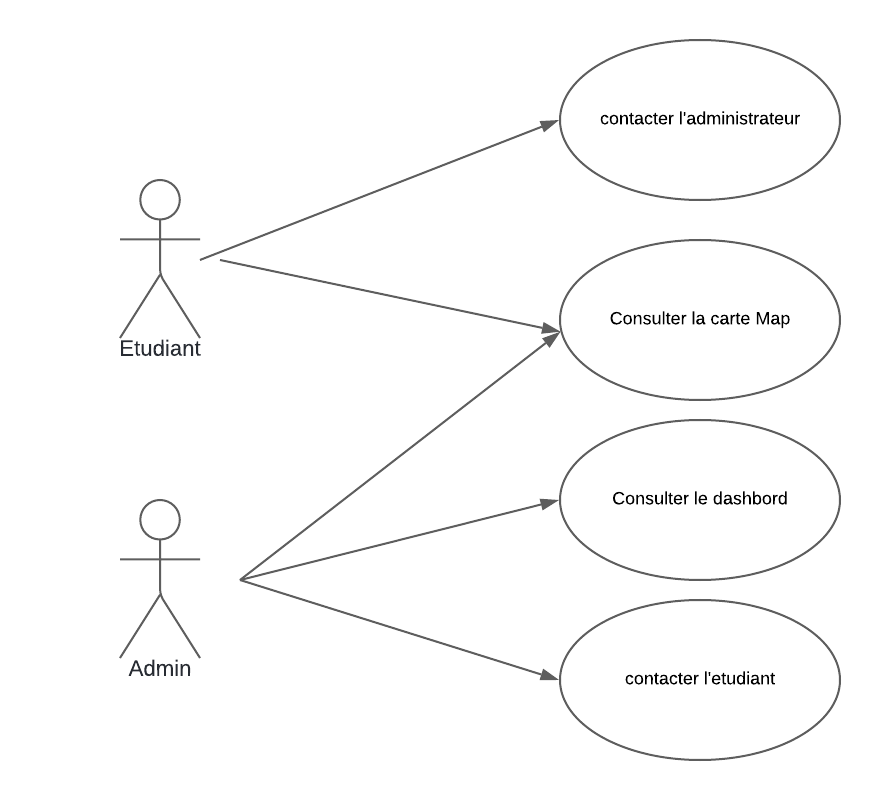
\includegraphics[height=6cm,width=12cm]{images/diagramme de cas d'utilisation 5eme sprint.png}%
    }
    \caption{Diagramme de cas d'utilisation Sprint 5 }
\end{figure}
\vspace{-9mm}
\subsection{Description textuelle du cas d’utilisation «Envoyer un message à l'administrateur»}
\vspace{-4mm}
Le tableau ci-dessous détaille le cas d'utilisation "Envoyer un message à l’administrateur" dans le cadre d'un système où les étudiants peuvent contacter l'administrateur après s'être connectés.

\begin{table}[h]
\centering
\begin{tabular}{|p{3cm}|p{12cm}|}
\hline
\textbf{Cas d'utilisation } & Envoyer un message à l'administrateur \\
\hline
\textbf{Acteurs} & Étudiant \\
\hline
\textbf{Précondition} & Utilisateur connecté \\
\hline
\textbf{Postcondition} & Message envoyé à l'administrateur \\
\hline
\textbf{Scénario nominal} & 
\begin{enumerate}
    \item L'Étudiant est sur la page d'accueil.
    \item L'Étudiant clique sur le bouton « Contact ».
    \item Le système affiche le formulaire d'envoi de message à l'administrateur.
    \item L'Étudiant rédige son message.
    \item L'Étudiant envoie le message.
\end{enumerate} \\
\hline
\end{tabular}
\caption{Description du cas d’utilisation « Envoyer un message à l'administrateur »}
\end{table}
\vspace{-9mm}
\subsection{Description textuelle du cas d’utilisation «Envoyer un message à un Étudiant»}
\vspace{-4mm}
Le tableau ci-dessous détaille le cas d'utilisation "Envoyer un message à un Étudiant" dans un système où les administrateurs peuvent contacter des étudiants spécifiques après s'être authentifiés.
\vspace{-3mm}
\begin{table}[h]
\centering
\begin{tabular}{|p{3cm}|p{12cm}|}
\hline
\textbf{Cas d'utilisation } & Envoyer un message  \\
\hline
\textbf{Acteurs} &  Admin \\
\hline
\textbf{Précondition} & Admin authentifié \\
\hline
\textbf{Postcondition} &   Étudiant connecté\\
\hline
\textbf{Scénario nominal} &
\begin{enumerate}
   \item L'administrateur est sur la page Dashboard.
    \item L'administrateur clique sur le bouton "Contacter".
    \item L'administrateur choisit l'étudiant à contacter..
    \item Le système affiche le formulaire d'envoi de message à l'administrateur.
    \item L'administrateur rédige son message.
    \item L'administrateur envoie le message.
\end{enumerate} \\
\hline
\end{tabular}
\caption{Description du cas d’utilisation «Envoyer un message à un Étudiant »}
\end{table}
\vspace{-1.9cm}
\section{Diagramme de séquence }
\vspace{-4mm}
Les diagrammes de séquence pour ce sprint se concentrent sur la fonctionnalité de chat, illustrant le processus par lequel les utilisateurs peuvent échanger des messages en temps réel avec d'autres utilisateurs ou avec l'administrateur de l'application, facilitant ainsi la communication et la résolution des problèmes de manière efficace.
\vspace{-1cm}
\subsection{Diagramme  de séquence <<Contacter un étudiant>> }

\vspace{-4mm}

Le diagramme de séquence "Contacter un étudiant" présente le processus par lequel un administrateur peut contacter un étudiant via l'application web, en initiant une interaction qui permet d'envoyer un message direct à un étudiant spécifique.

\begin{figure}[H]%
    \center%
    \setlength{\fboxsep}{5pt}%
    \setlength{\fboxrule}{0.5pt}%
    \fbox{
    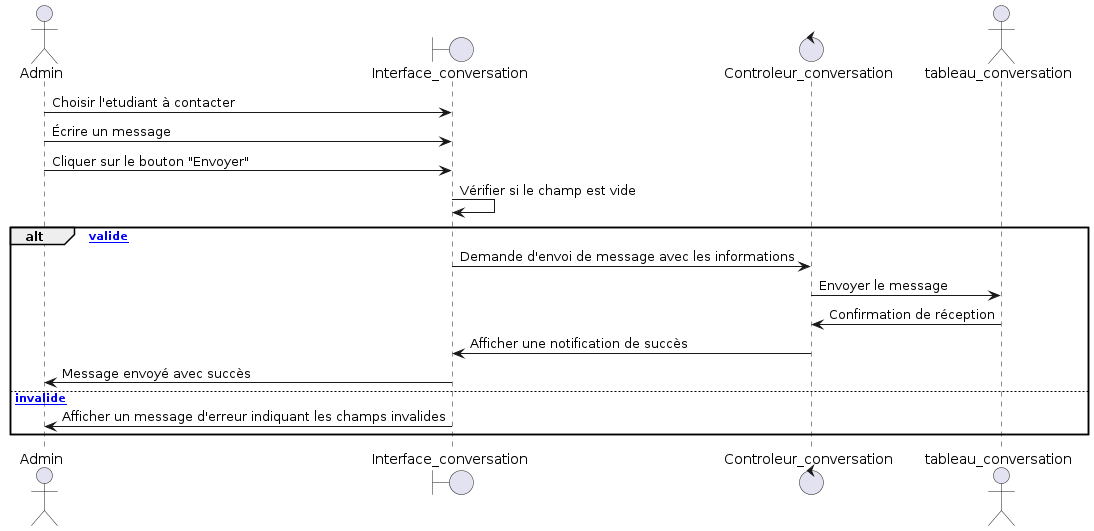
\includegraphics[height=7cm,width=15cm]{images/admintoetudiant.png}%
    }
    \caption{Diagramme de cas d'utilisation }
\end{figure}
\vspace{-4mm}
\subsection{Diagramme de séquence <<Contacter admin>> }
\vspace{-4mm}
Le diagramme de séquence "Contacter l'administrateur" illustre le processus par lequel un utilisateur peut contacter l'administrateur de l'application via l'interface de communication dédiée, permettant ainsi d'envoyer un message direct à l'administrateur pour poser des questions, signaler des problèmes ou demander de l'aide.

\begin{figure}[H]%
    \center%
    \setlength{\fboxsep}{5pt}%
    \setlength{\fboxrule}{0.5pt}%
    \fbox{
    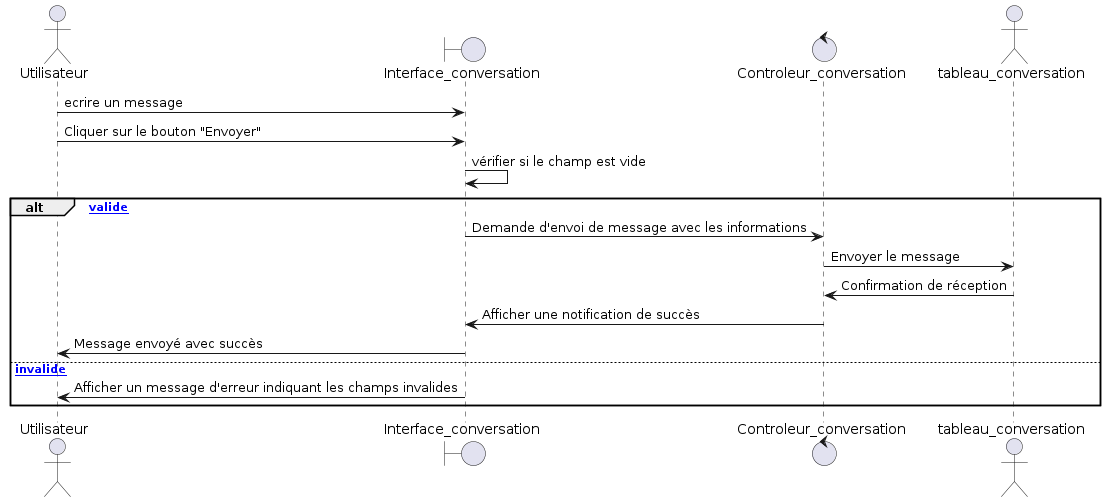
\includegraphics[height=12cm,width=15cm]{images/lasstcontact.png}%
    }
    \caption{Diagramme de séquence <<Contacter admin>> }
\end{figure}


\vspace{-9mm}


\section{Diagramme de classes }
\vspace{-4mm}
Le diagramme de classes pour la gestion de la carte, du chat et du tableau de bord dans notre système offre une représentation structurée des entités et des fonctionnalités associées. Chaque classe, comme "Carte", "Chat" et "Tableau de bord", est conçue pour gérer les opérations spécifiques liées à sa fonctionnalité respective. 
\vspace{-4mm}
\begin{figure}[H]%
    \center%
    \setlength{\fboxsep}{5pt}%
    \setlength{\fboxrule}{0.5pt}%
    \fbox{
    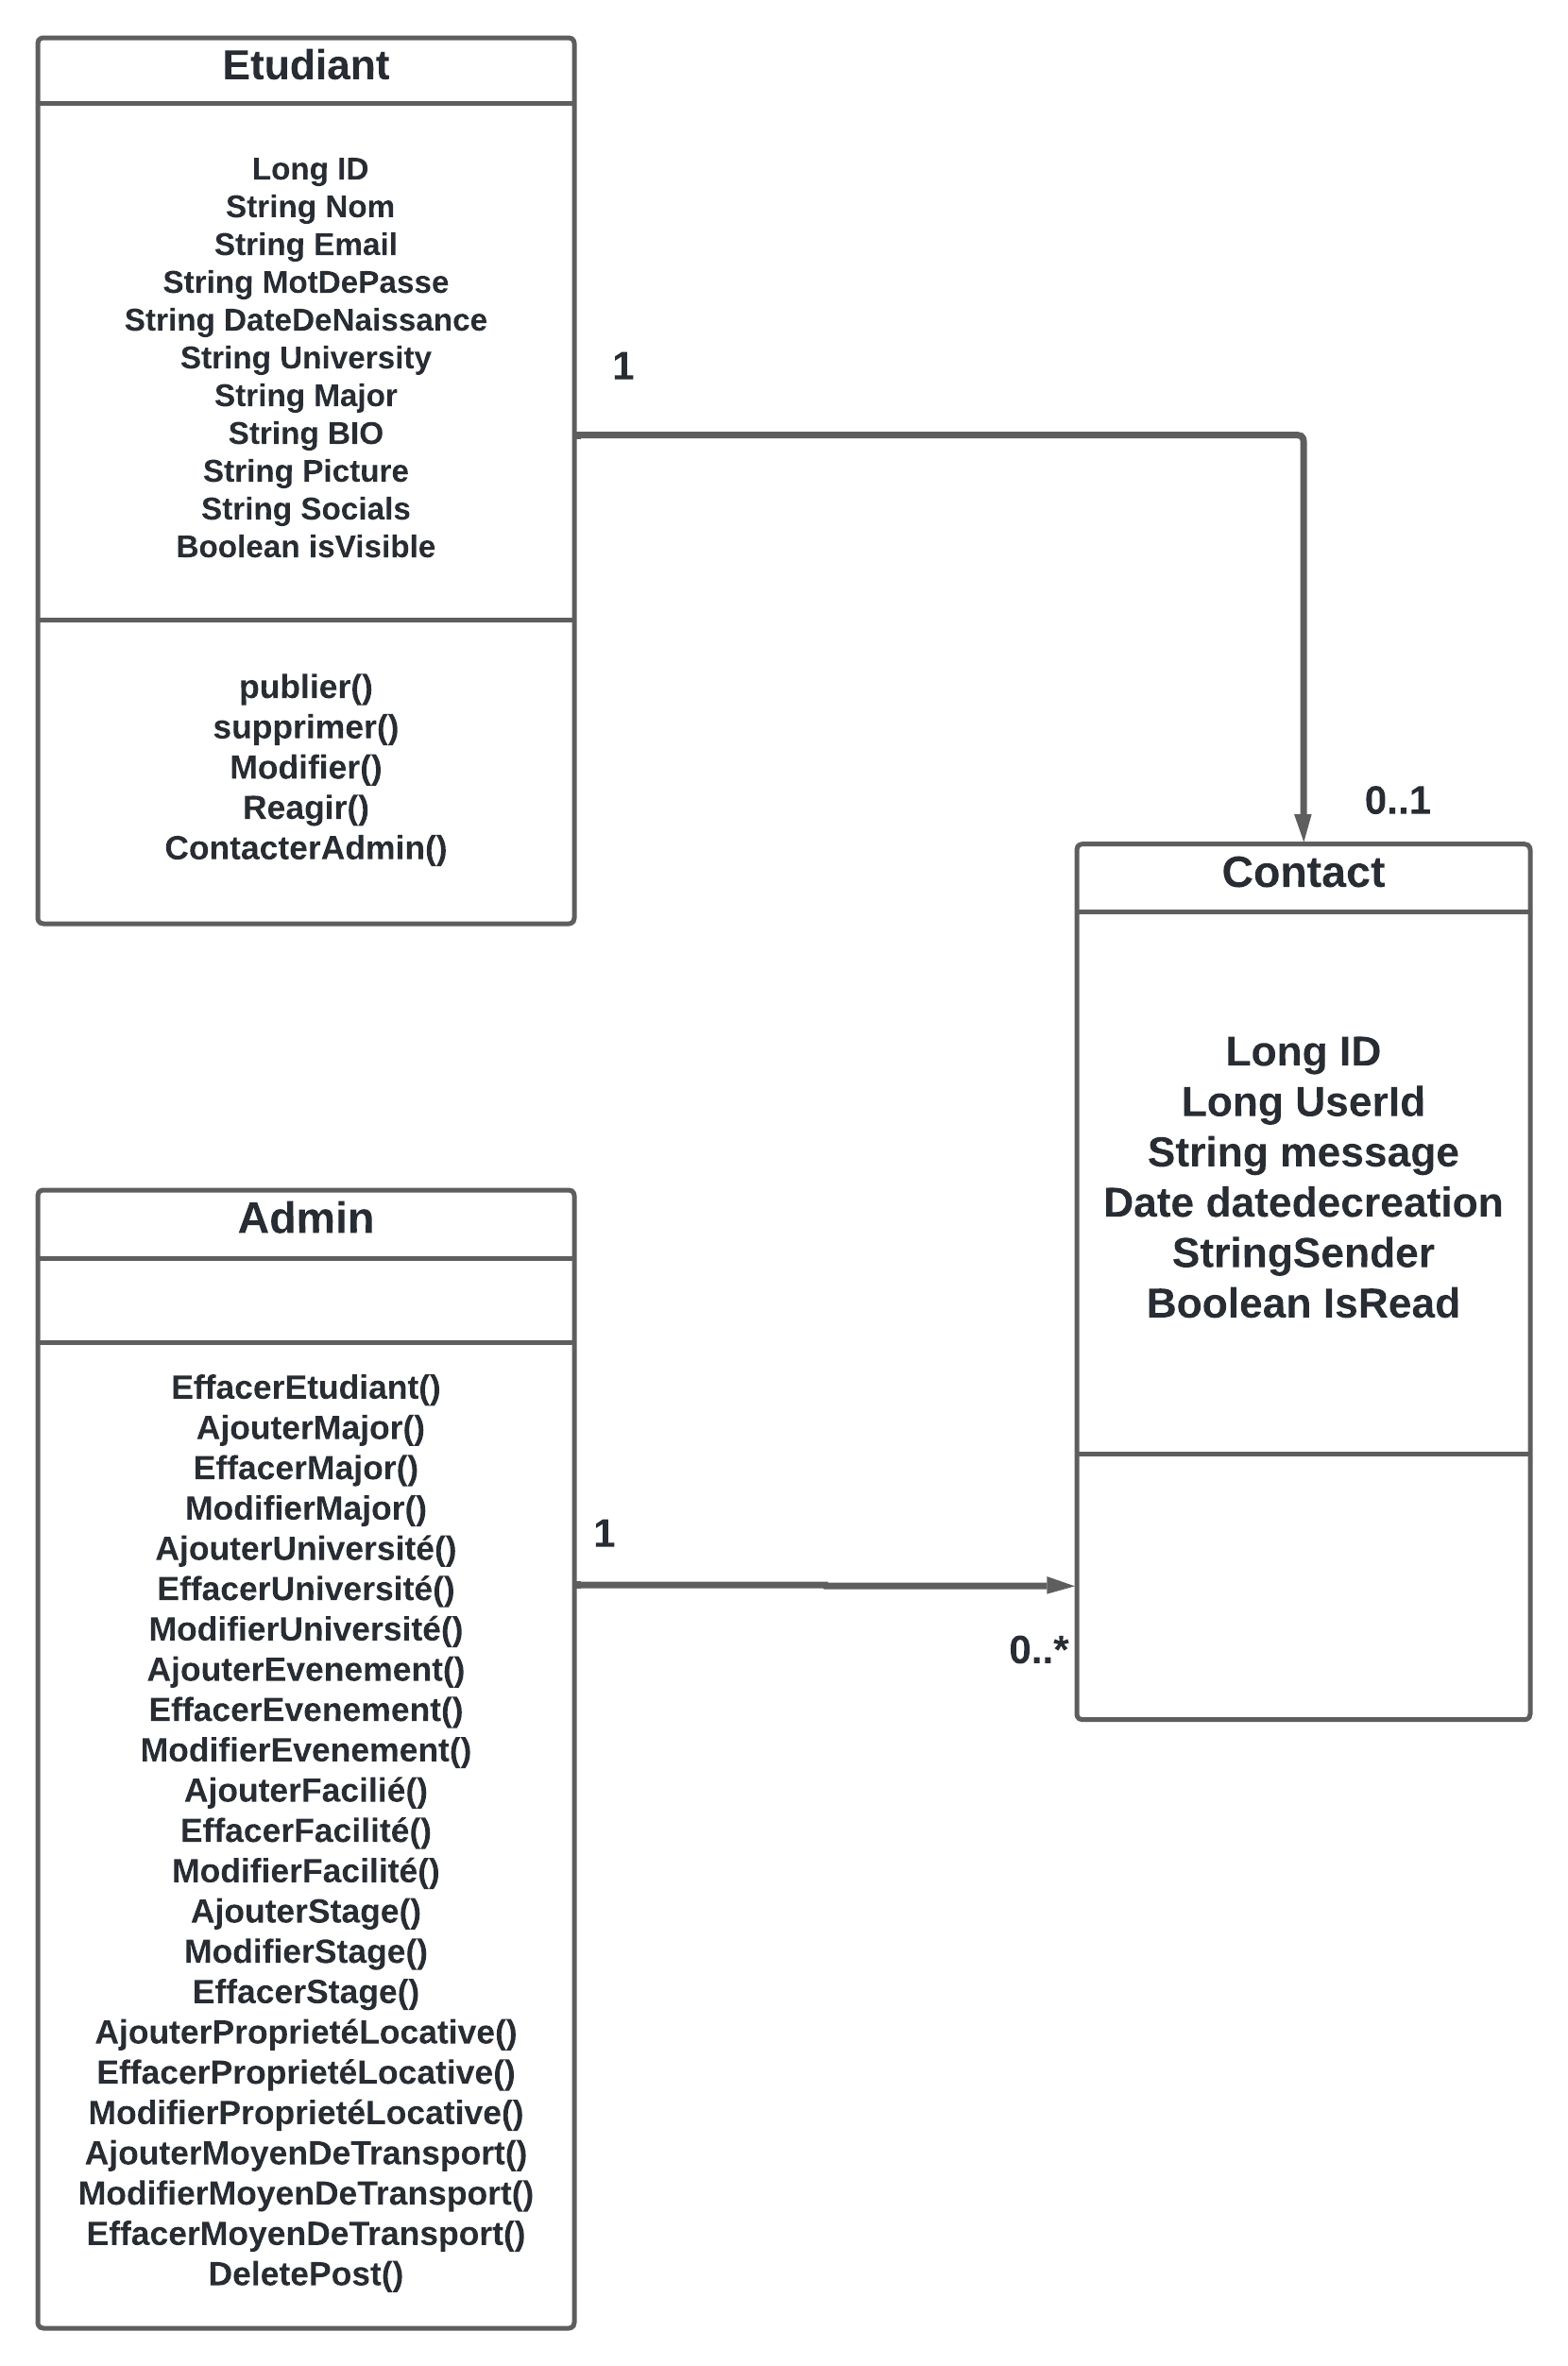
\includegraphics[height=13cm,width=15cm]{images/Diagramme de classe contact (2).png}%
    }
    \caption{Diagramme de classes sprint 5 }
\end{figure}
\vspace{-1.2cm}
\section{Réalisation }
\vspace{-4mm}
La partie de réalisation représente la dernière phase du cycle de développement d’un sprint. Elle permet de présenter les résultats obtenus lors de l’étape de développement afin d’assurer et de garantir une version de qualité. Nous allons montrer cela par des captures d’écrans des fonctionnalités ayant été développées.
\vspace{-1cm}
\section{Contact administrateur}
\vspace{-4mm}
L'interface "Contacter l'administrateur" dans la partie mobile permet aux utilisateurs d'envoyer des messages directement à l'administrateur. Les utilisateurs peuvent rédiger leur message et l'envoyer en un clic, facilitant ainsi une communication directe et efficace avec l'administration.
\vspace{-4mm}
\begin{figure}[H]%
    \center%
    \setlength{\fboxsep}{5pt}%
    \setlength{\fboxrule}{0.5pt}%
    \fbox{
    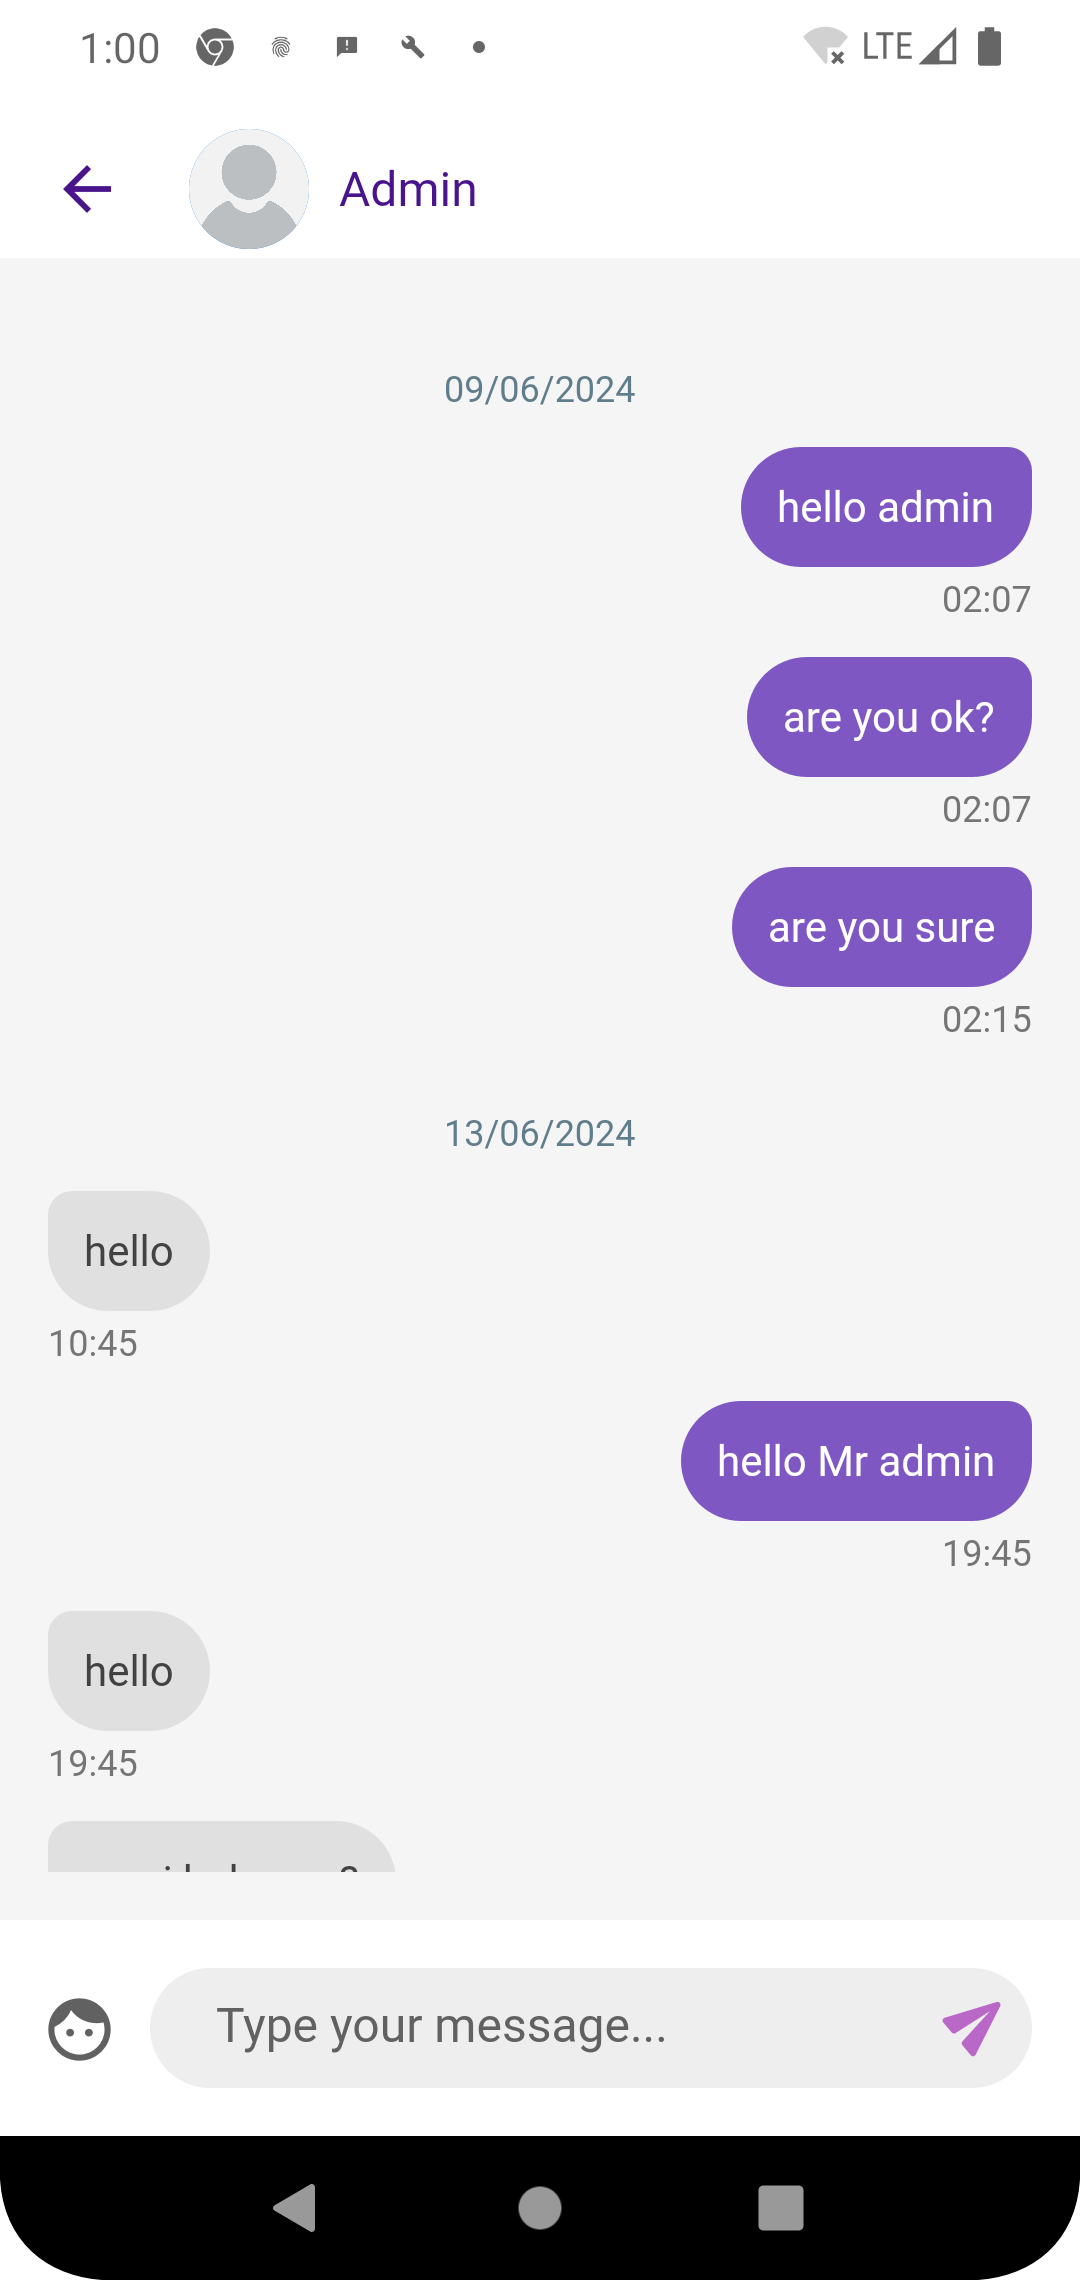
\includegraphics[height=10cm,width=7cm]{images/XChatPage.png}%
    }
    \caption{Interface Contacter administrateur  }
\end{figure}
\vspace{-1.5cm}
\section{Contact Utilisateur }
\vspace{-4mm}
L'interface web pour l'administrateur facilite la communication avec les utilisateurs. Elle offre une section dédiée où l'administrateur peut sélectionner des utilisateurs spécifiques, rédiger un message, et l'envoyer directement, assurant ainsi une communication efficace et directe.

\begin{figure}[H]%
    \center%
    \setlength{\fboxsep}{5pt}%
    \setlength{\fboxrule}{0.5pt}%
    \fbox{
    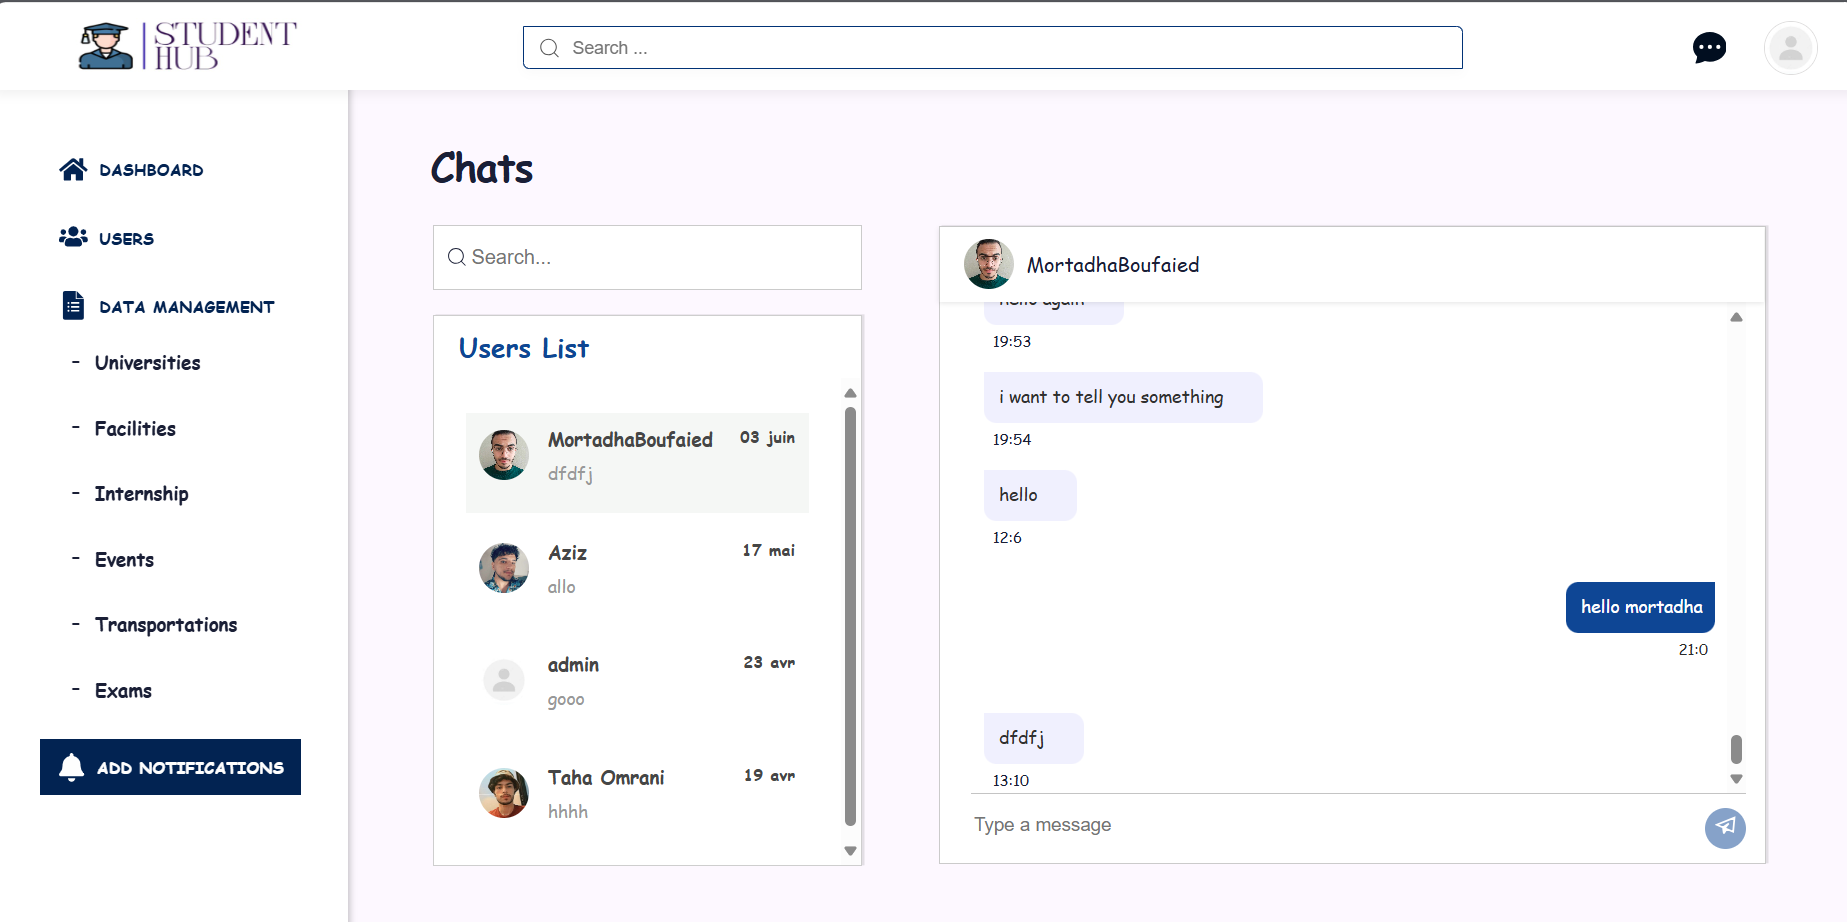
\includegraphics[height=8cm,width=15.5cm]{images/AAAChat.png}%
    }
\end{figure}
\vspace{-7mm}
\vspace{-4mm}
\begin{figure}[H]%
    \center%
    \setlength{\fboxsep}{5pt}%
    \setlength{\fboxrule}{0.5pt}%
    \fbox{
    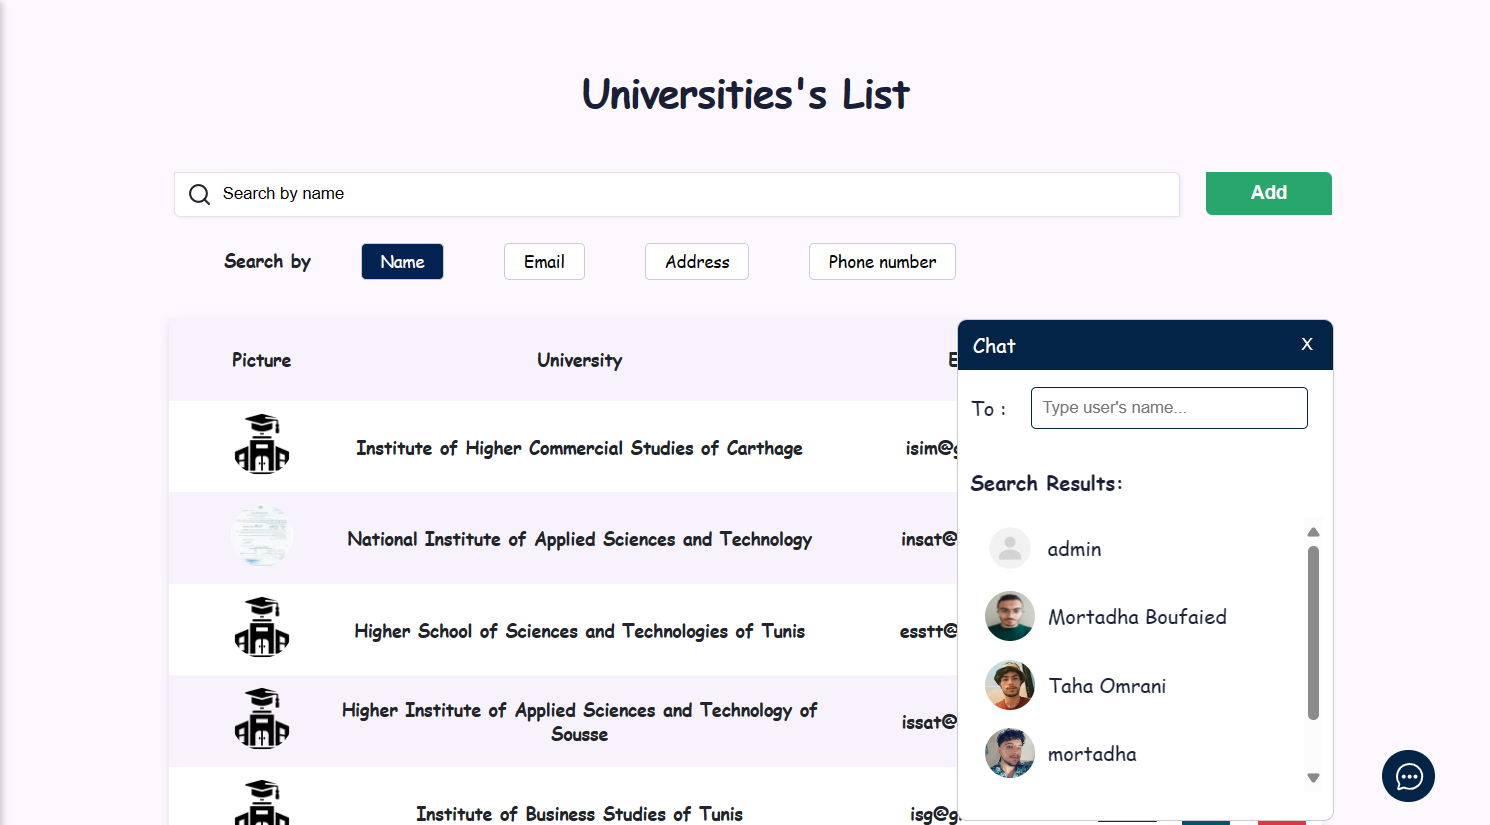
\includegraphics[height=8cm,width=15.5cm]{images/MiniChat.png}%
    }
    \caption{Interface Contacter un utilisateur  }
\end{figure}

\vspace{-1.2cm}

\section{Le Dashbord d'administrateur }
\vspace{-4mm}
Le tableau de bord de l'administrateur dans la partie web se concentre principalement sur la présentation des graphiques et des statistiques clés. Il offre une vue visuelle des données importantes telles que le nombre d'utilisateurs, les événements à venir, les publications récentes, etc. Ces graphiques permettent à l'administrateur de suivre facilement les tendances et les performances de l'application, ce qui facilite la prise de décision et la planification stratégique.

\begin{figure}[H]%
    \center%
    \setlength{\fboxsep}{5pt}%
    \setlength{\fboxrule}{0.5pt}%
    \fbox{
    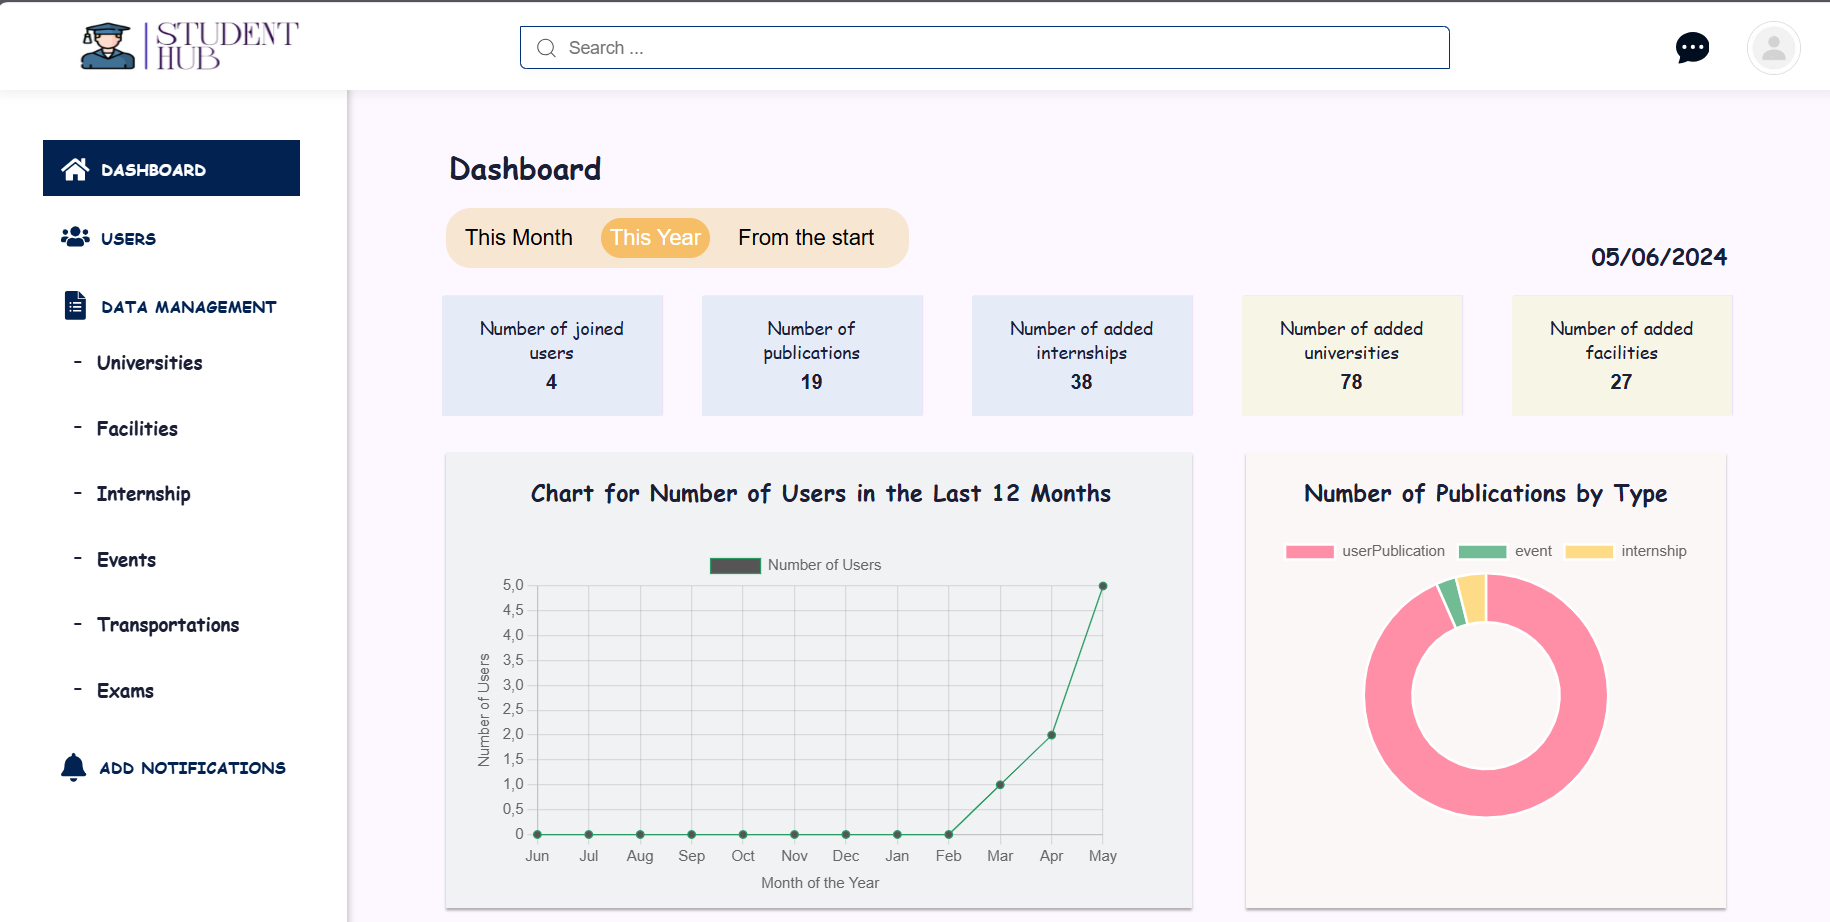
\includegraphics[height=8cm,width=15.5cm]{images/AAADashboard.png}%
    }
    \caption{Interace tableau de bord  }
\end{figure}

\section{La carte map }
\vspace{-4mm}
La carte interactive dans notre application mobile affiche la localisation des différentes Endroits disponibles pour les utilisateurs. En utilisant des marqueurs sur la carte, les utilisateurs peuvent visualiser facilement les emplacements des universités, des stations de transport, des lieux d'événements, et d'autres installations pertinentes. Cette fonctionnalité offre une expérience conviviale aux utilisateurs, leur permettant de naviguer efficacement dans leur environnement et de trouver les services qui les intéressent.

\begin{figure}[H]%
    \center%
    \setlength{\fboxsep}{5pt}%
    \setlength{\fboxrule}{0.5pt}%
    \fbox{
    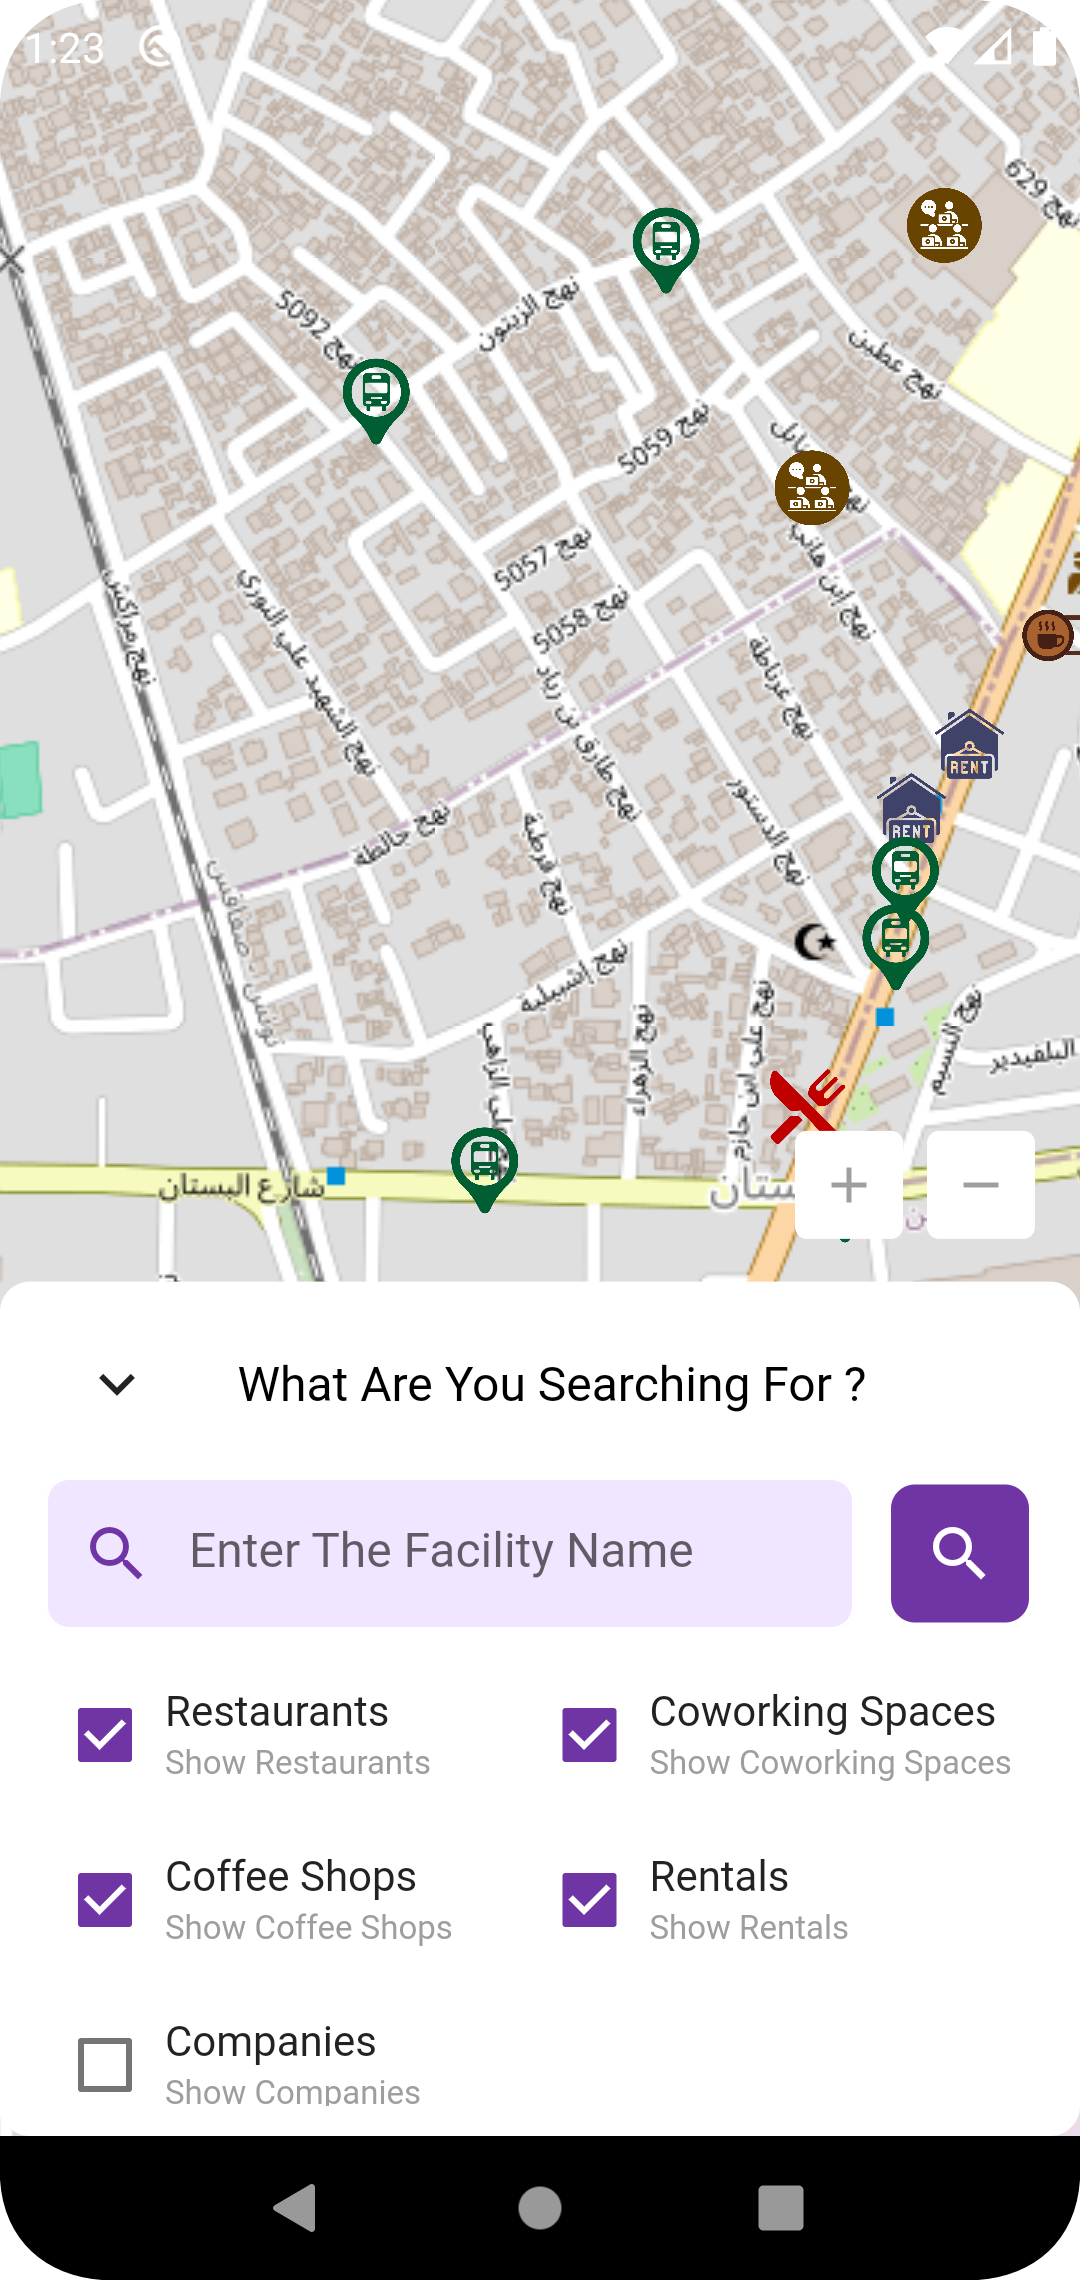
\includegraphics[height=10cm,width=7cm]{images/AAAMap.png}%
    }
    \caption{Interface carte map }
\end{figure}
\vspace{-1.2cm}
\section{Conclusion }
\vspace{-4mm}
En conclusion, ce sprint a été dédié à l'amélioration de la gestion des publications et des notifications au sein de notre application. En fournissant aux administrateurs des outils performants et intuitifs, notre objectif est de rehausser l'expérience utilisateur en optimisant la visibilité et la gestion des publications, ainsi qu'en rendant les notifications plus pertinentes et réactives. Ce sprint marque une étape importante dans notre engagement à offrir une plateforme dynamique et engageante pour nos utilisateurs

\end{sloppypar} 
